\documentclass[xcolor={usenames,dvipsnames,svgnames}, compress]{beamer}

\usepackage{booktabs}
\usepackage{dcolumn}
\usepackage{colortbl}
\usepackage{ifxetex}
\usepackage{amsmath}
\usepackage[style=authoryear-comp]{biblatex}
\usepackage[no-math]{fontspec}

\definecolor{untractable_red}{RGB}{209, 25, 25}
\definecolor{tractable_green}{RGB}{0, 153, 51}

\newcommand{\argmax}{\operatornamewithlimits{argmax}}

\usetheme{enziteto}

\setbeamertemplate{headline}{}

\addbibresource{../referomnia/referomnia.bib}

\title{Learning Sum-Product Networks}
\author{Nicola Di Mauro \and Antonio Vergari}
% \date{September 2016}
\institute{Università degli Studi di Bari}
\department{Dipartimento di Informatica}
\laboratory{LACAM}
\group{Machine Learning}
\institutelogo{
\includegraphics[width=25pt]{figures/unibaba}}
\lablogo{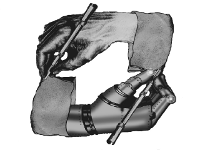
\includegraphics[width=35pt]{figures/lacam}}

\footnotesize \let\small\footnotesize

\begin{document}

\begin{frame}
  \setbeamertemplate{headline}{}
  \setbeamertemplate{footline}{}
  \titlepage
\end{frame}


\begin{frame}[t]
  \frametitle{The need for SPNs}
  \framesubtitle{Why should you work on SPNs?}
\begin{itemize}
\item exact tractable inference
  \item NN for which structure learning is easy
\end{itemize}
\end{frame}

\section{Representation}
{\setbeamertemplate{headline}{}
  \begin{frame}
    \sectionpage
  \end{frame}
}

\begin{frame}
  \frametitle{Density estimation}
\end{frame}

\begin{frame}
  \frametitle{(Different kinds of) Inference}
\end{frame}

\begin{frame}
  \frametitle{Tractable Probabilistic Models}
\end{frame}

\begin{frame}
  \frametitle{Sum-Product Networks}
\end{frame}

\begin{frame}
  \frametitle{Scopes}
\end{frame}

\begin{frame}
  \frametitle{Structural Properties}
\end{frame}

\section{Inference}
{\setbeamertemplate{headline}{}
  \begin{frame}
    \sectionpage
  \end{frame}
}

\begin{frame}
  \frametitle{Complete evidence}
\end{frame}

\begin{frame}
  \frametitle{Marginal inference}
\end{frame}

\begin{frame}
  \frametitle{MPE inference}
\end{frame}


\section{Interpretation}
{\setbeamertemplate{headline}{}
  \begin{frame}
    \sectionpage
  \end{frame}
}

\begin{frame}
\frametitle{Interpretation}
\begin{itemize}
\item probabilistic model
\item deep feedforward neural network
\end{itemize}
\end{frame}


\begin{frame}
\frametitle{Network Polynomials}
\end{frame}

\begin{frame}
  \frametitle{Arithmetic Circuits}
  Differences with ACs:
  \begin{itemize}
  \item probabilistic semantics
    \begin{itemize}
    \item learning
      \item sampling
    \end{itemize}
    \item no shared weights
  \end{itemize}
\end{frame}

\begin{frame}
  \frametitle{SPNs as BNs I}
  Zhao
\end{frame}

\begin{frame}
  \frametitle{SPNs as BNs II}
  Peharz
\end{frame}


\section{Learning}
{\setbeamertemplate{headline}{}
  \begin{frame}
    \sectionpage
  \end{frame}
}

\begin{frame}
  \frametitle{Structure Learning}
\end{frame}

\begin{frame}
  \frametitle{LearnSPN}
\end{frame}

\begin{frame}
  \frametitle{LearnSPN-b}
\end{frame}

\begin{frame}
  \frametitle{New Structure Learning Tendencies}
\end{frame}

\begin{frame}
\frametitle{Parameter Learning}
\end{frame}

\begin{frame}
  \frametitle{Hard/Soft Parameter Learning}
\end{frame}

\begin{frame}
  \frametitle{Bayesian Parameter Learning}
\end{frame}

\begin{frame}
  \frametitle{Parameter Learning VS LearnSPN}
  Collapsed Variational Inference is useless : D
\end{frame}

\section{Representation Learning}
{\setbeamertemplate{headline}{}
  \begin{frame}
    \sectionpage
  \end{frame}
}

\begin{frame}
  \frametitle{Extracting Embeddings}
\end{frame}

\begin{frame}
  \frametitle{Classification}
\end{frame}

\begin{frame}
  \frametitle{Filtering Embeddings}
\end{frame}

\begin{frame}
  \frametitle{Random Marginal Queries}
\end{frame}

\begin{frame}
  \frametitle{Encoding/Decoding Embeddings}
  MPN as autoencoders\footnotenomarkleft{Vergari et al. Encoding and Decoding
    Representations with Sum-Product Networks, 2016, to appear}.
\end{frame}




\section{Applications}
{\setbeamertemplate{headline}{}
  \begin{frame}
    \sectionpage
  \end{frame}
}

\begin{frame}
  \frametitle{Applications I: computer vision}
\end{frame}


\begin{frame}
\frametitle{Applications II: language modeling}
\end{frame}

\begin{frame}
  \frametitle{Applications III: activity recognition}
\end{frame}

\begin{frame}
  \frametitle{Applications IV: speech}
\end{frame}


\begin{frame}
\frametitle{Trends \& What to do next}
\end{frame}

\section{References}
{\setbeamertemplate{headline}{}
  \begin{frame}
    \sectionpage
  \end{frame}
}

\begin{frame}
  \frametitle{awesome-spn}
  A curated and structured list of resources about SPNs\footnote{Inspired by the \href{SPN page}{http://spn.cs.washington.edu/} at the Washington University}.\par
  \url{https://github.com/arranger1044/awesome-spn}
\end{frame}

\begin{frame} [allowframebreaks]
  \setbeamertemplate{bibliography item}{}
  \setlength\bibitemsep{8pt}
  \printbibliography
\end{frame}

\end{document}
%%% Local Variables:
%%% mode: latex
%%% TeX-master: t
%%% TeX-engine: xetex
%%% End:
